%!TEX root = ../../main.tex

\chapter{Proposed method} \label{chap:method}
    \section{Introduction}
        This chapter represents the methodology proposed in this thesis.
        Section \ref{sec:general_framework} gives an overview of the multi-view human action and gesture recognition framework.
        Section \ref{sec:feature_extraction} provides the details on different CNN architectures used in feature extraction for individual view.
        Section \ref{sec:common_feature_space} describes the proposed improvement of MvDA for building common feature space across multiple views.

    %!TEX root = ../../main.tex

\section{General Framework} \label{sec:general_framework}
    We propose a framework for cross-view action recognition as illustrated in Figure \ref{fig:frw}. It composes of two phases: training phase and recognition phase. 
    \begin{itemize}
        \item \textbf{Training phase}: Suppose we have $v$ views. The training phase consists of three main steps: 
        \begin{enumerate}
            \item \textit{Feature extraction at separated view}: All training samples from each separated view will be passed though a feature extraction step. Different deep techniques will be investigated, including 2D CNNs based feature extraction combined with aggregation techniques and 3D CNNs based feature extraction, to output the final descriptor for each video sample. Let's call the features extracted at this step as features at single views or separated view features. 
            \item \textit{Common space construction}: This step builds a common feature space so that samples belonging to the same class will be close to each other even they are captured from different viewpoints. It takes all separated view features extracted from training set from the previous step and find a set of $v$ linear transformations $({\omega}_1, {\omega}_2, ..., {\omega}_v)$ that minimize within-class variation while maximizing between-class variation of features in the projected space (common space). 
            \item \textit{Training classifier}: Once $v$ transformations have been computed, the projected features in the common space of each view will be utilized to train a simple predictive model $F$ (i.e. kNN).
        \end{enumerate}
        \item \textbf{Recognition phase}. Multi-view recognition consists of two following steps:
        \begin{enumerate}
            \item \textit{Feature extraction} Features of the testing sample $x_j$ from the view $V_j$ are extracted. This feature will be projected in the pre-built common space by the corresponding transformation ${\omega}_j$. The projected feature is denoted as $y_j = {\omega}^T_j*x_j$.
            \item \textit{Class prediction}: The projected feature $y_j$ will be passed into the classifier $F(y_j)$ that outputs the label of action.
        \end{enumerate}
    \end{itemize}

    \begin{figure}[htbp]
        \centering
        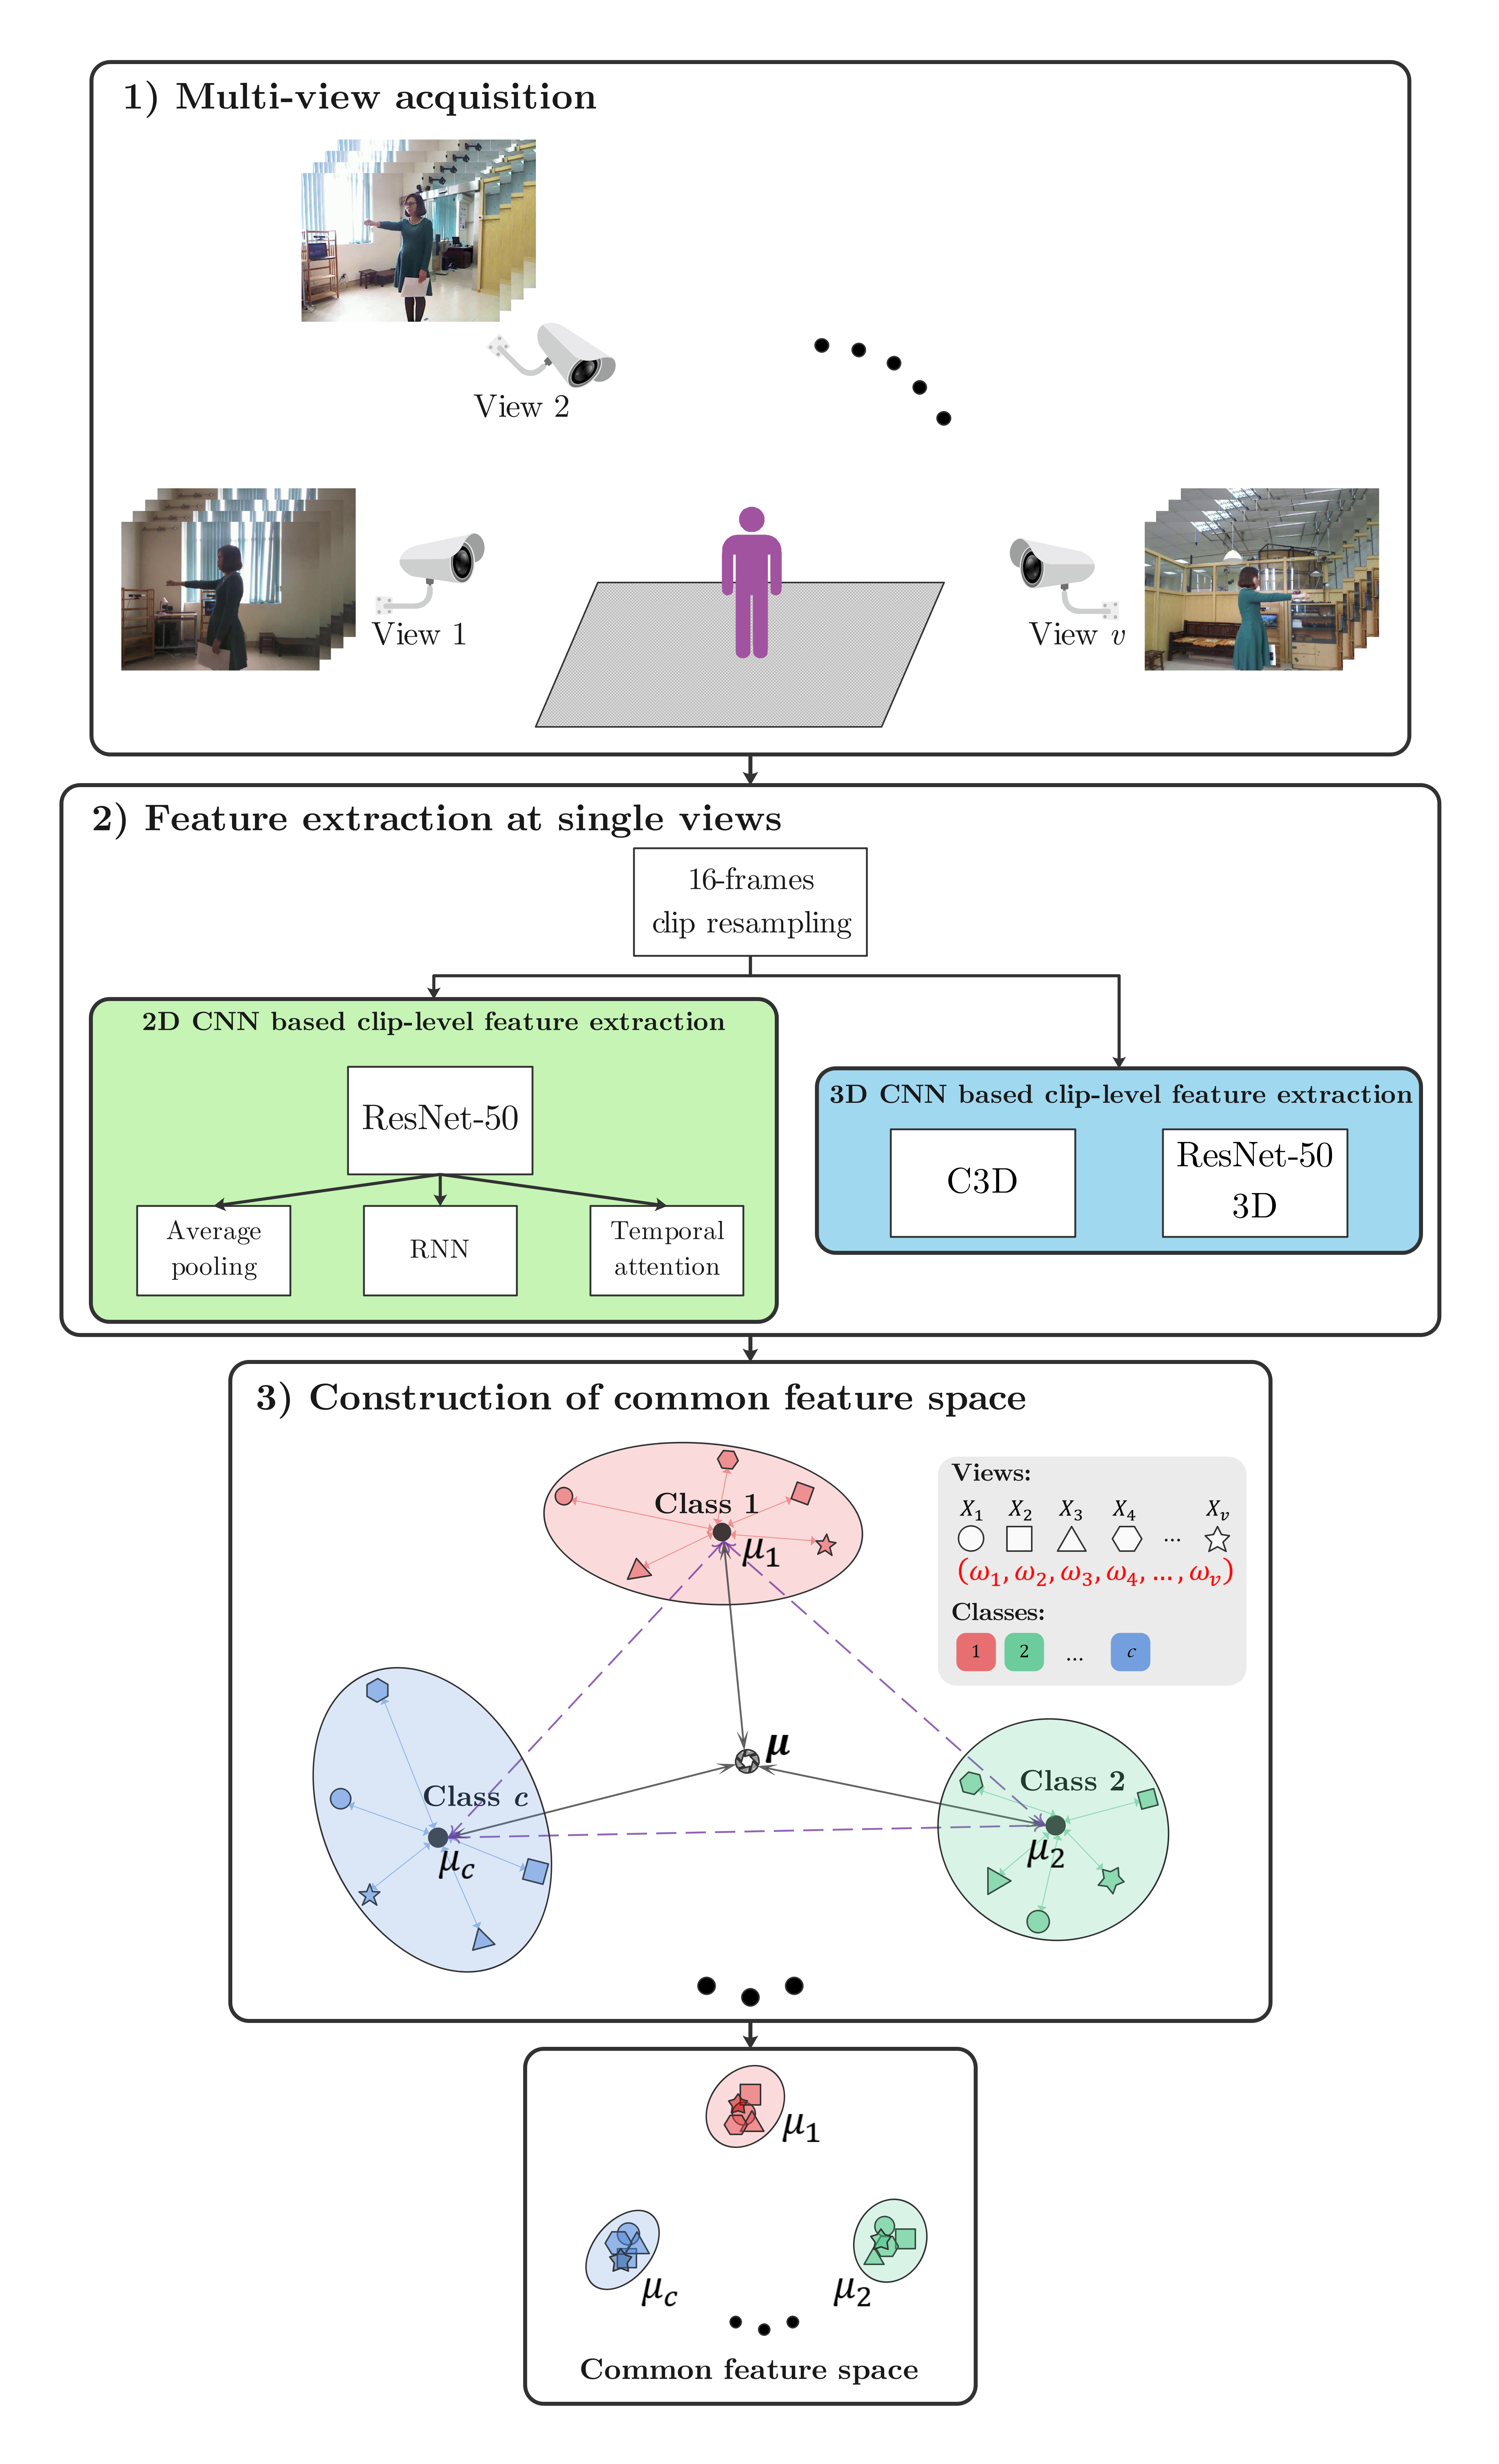
\includegraphics[width=0.85\linewidth]{figs/Framework.png}
        \caption{Proposed framework for building common feature space with pairwise-covariance multi-view discriminant analysis (pc-MvDA).}
        %\vspace{-0.3cm}
        \label{fig:frw}
    \end{figure}
    %In the following, I will detail the step of feature extraction at separated view in subsection \ref{sub:private}, the step of building the common feature space in subsection \ref{sub:common}. 

    %!TEX root = ../../../main.tex

\section{Feature extraction at individual view using deep learning techniques} \label{sec:private}
    %!TEX root = ../../../main.tex

\subsection{2D CNN based clip-level feature extraction}
    First, the ResNet-50 Convolution Neural Network \cite{he2016deep} is used as a 2D CNN network to extract spatial features of each frame in video. Fig.\ref{fig:resnet50} illustrates the architecture of ResNet-50 which composes of five convolutional blocks stacked on top of each other. The network is pre-trained on ImageNet then fine-tuned using training sets described in Section \ref{sec:experimentalresult}. Deep residual features are extracted from the output of the last convolutional block of the network which is a 2048-D feature vector. 
    \begin{figure}[htbp]
        \centering
        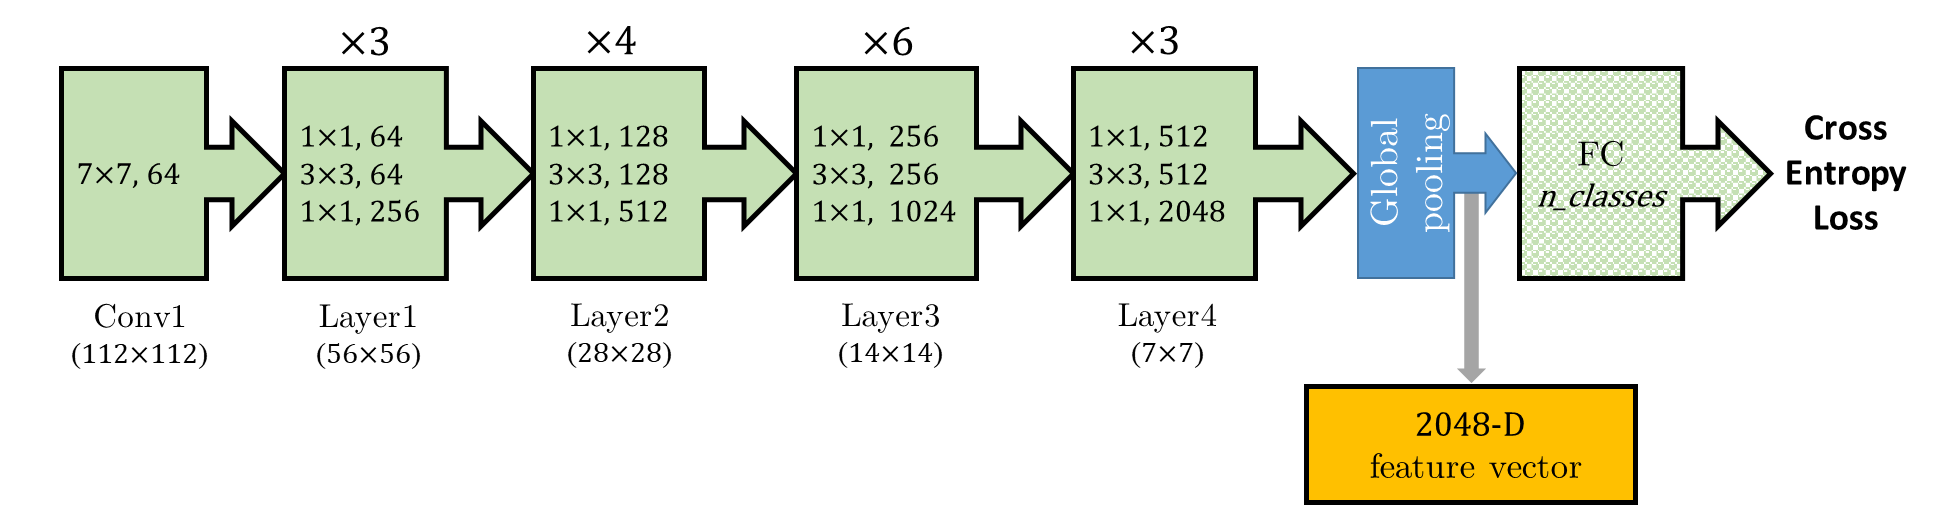
\includegraphics[width=1\linewidth]{Figs/Resnet50.png}
        \caption{Architecture of ResNet-50 utilized in our work for feature extraction at each separated view}
        %\vspace{-0.3cm}
        \label{fig:resnet50}
    \end{figure}
    We then aggregate frame-level features to create video-level features. In this work, we implement three temporal modeling techniques: 1) average pooling (AP); 2) recurrent neural network (RNN) and 3) temporal attention (TA). Fig.\ref{fig:pooling} illustrates three techniques.
    \begin{figure}[htbp]
        \centering
        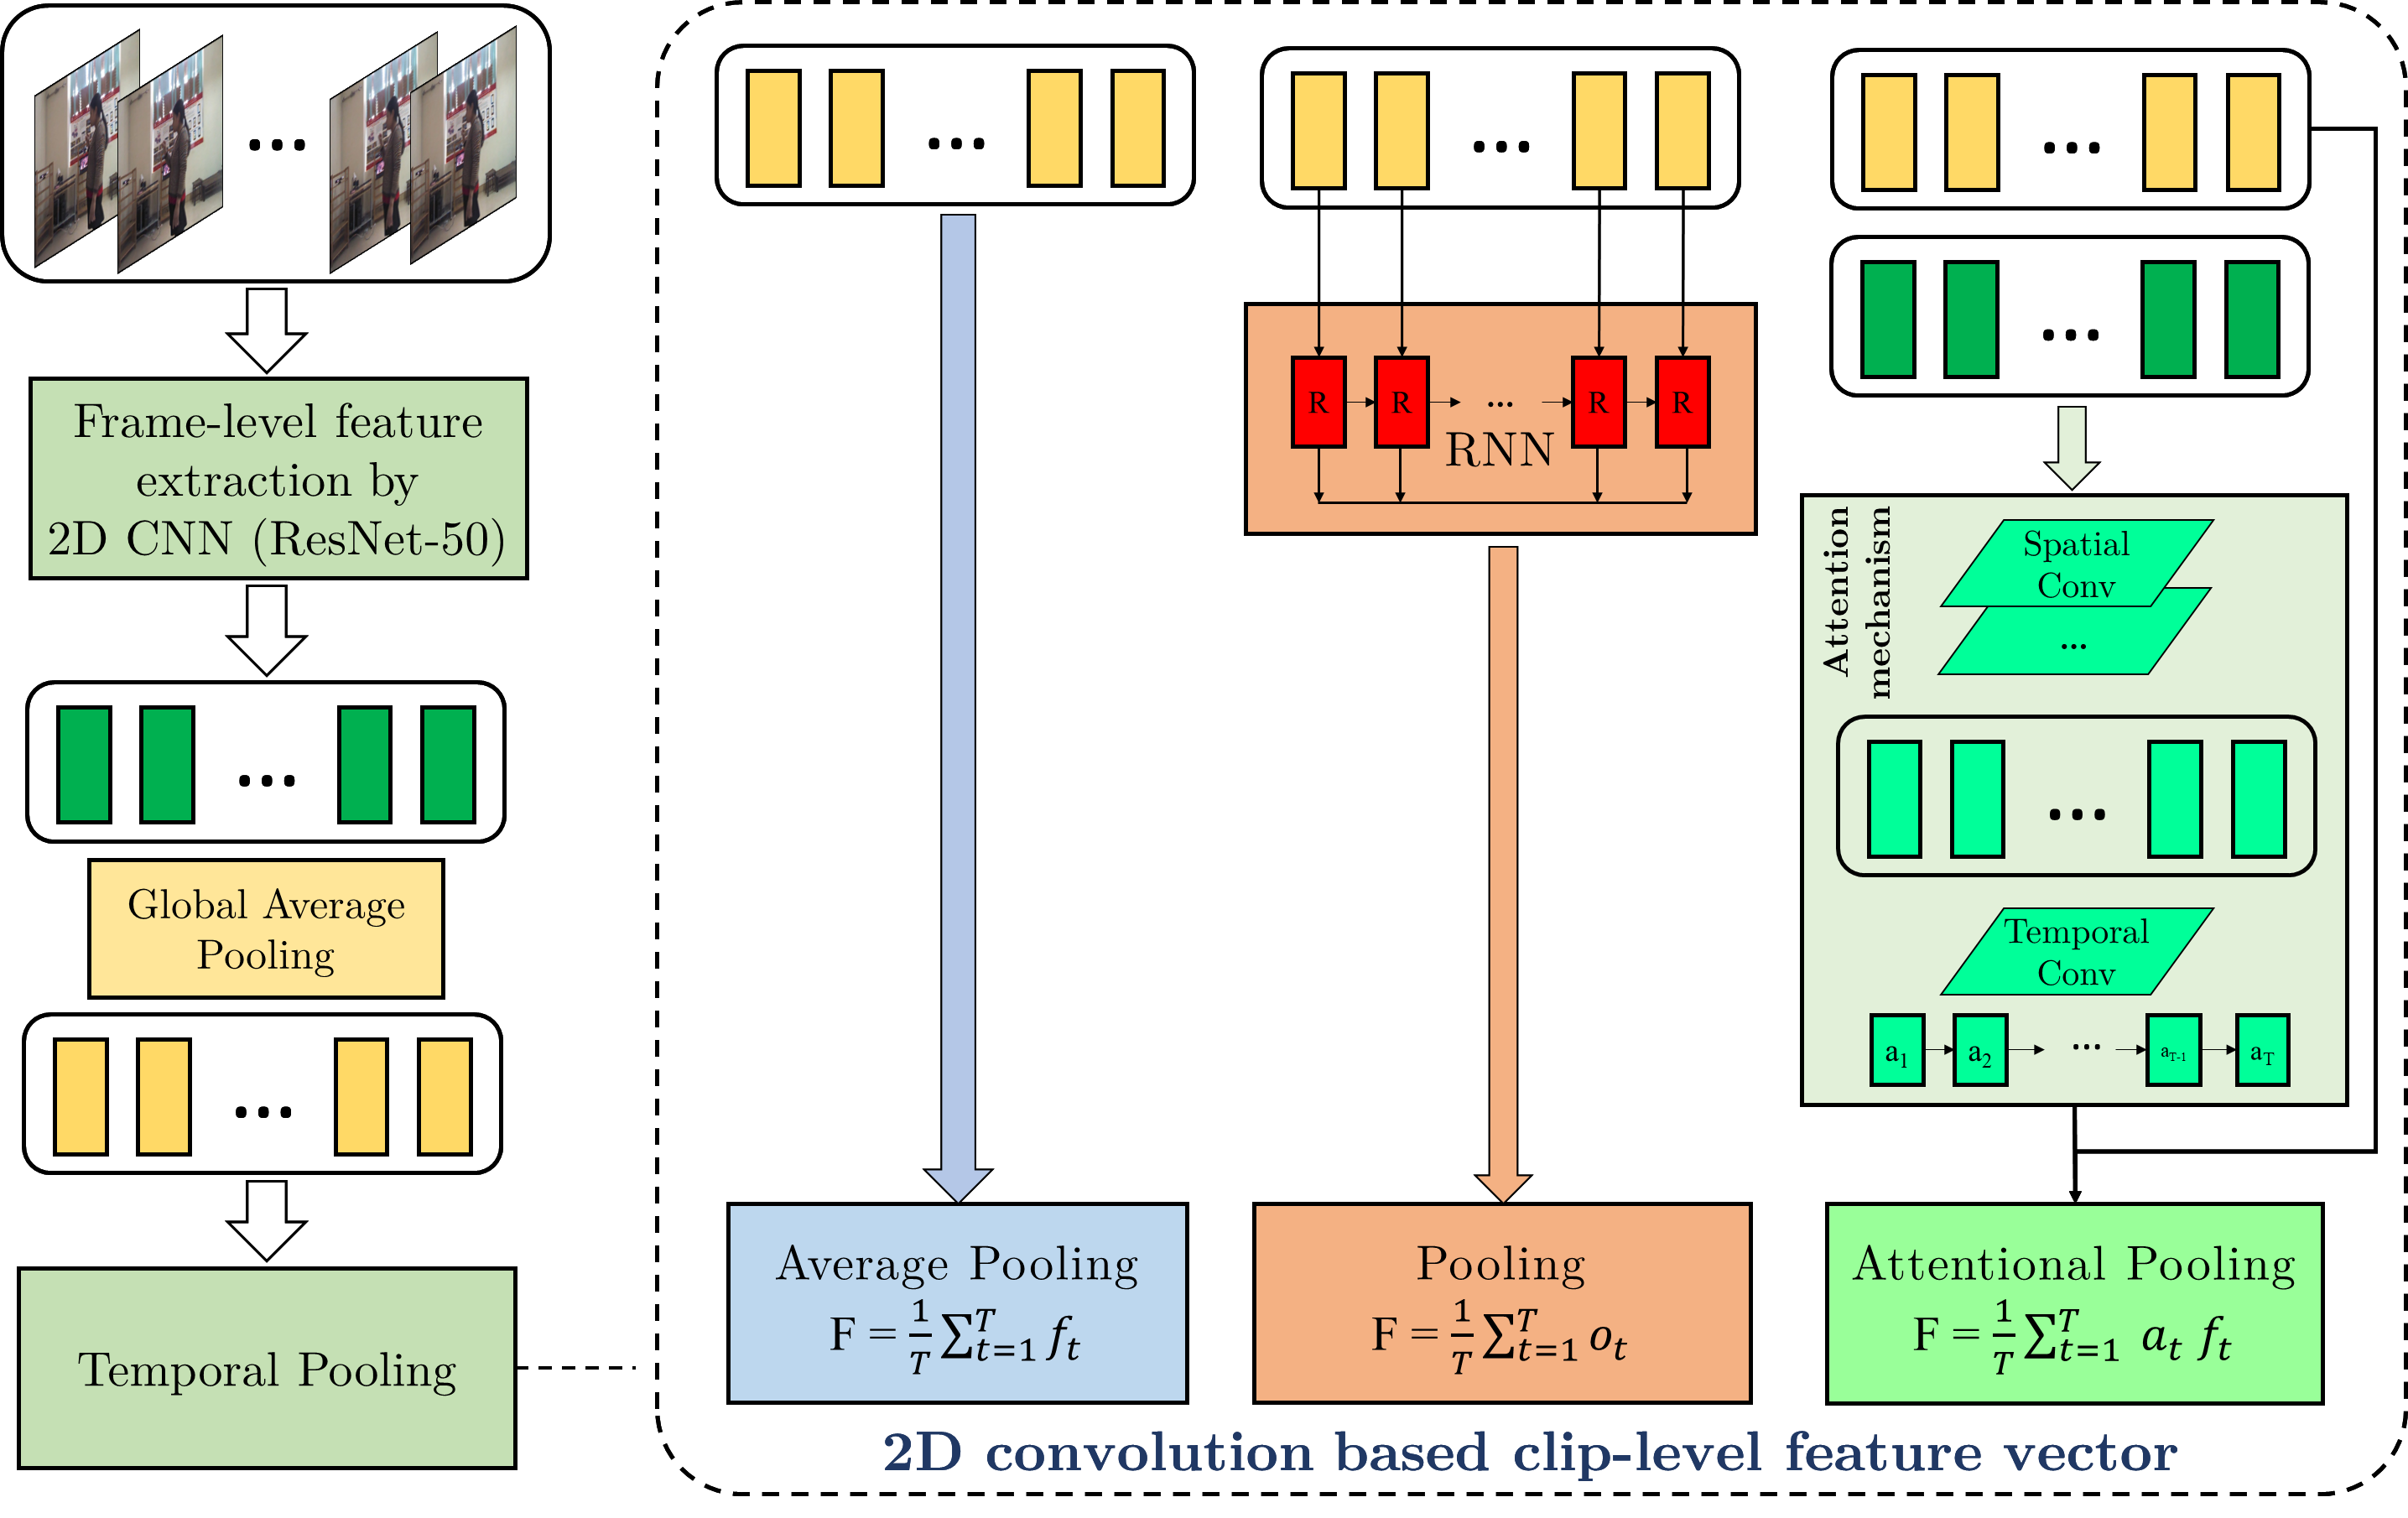
\includegraphics[width=1\linewidth]{Figs/Pooling.png}
        \caption{Three pooling techniques: Average Pooling (AP), Recurrent Neural Network (RNN) and Temporal Attention Pooling (TA)}
        %\vspace{-0.3cm}
        \label{fig:pooling}
    \end{figure}

    \textbf{Average Pooling - AP}: Let ${f}$ be the video-level feature, ${f_t}$ be the frame-level feature at time ${t}$, $T$ be the number of frames in video. Average pooling technique simply averages all frame-level features uniformly to create the video-level feature:
    \begin{equation}
    f=\frac{1}{T}\sum_{t=1}^T{f_t}
    \end{equation}
    As a frame-level feature is a 2048-D vector, the video-level feature is of the same dimension.\\
    \textbf{Recurrent Neural Network - RNN}: An RNN cell encodes a $t^{th}$ frame-level feature at time $t$ of the sequence and passes the hidden state $h_t$ into the next time step. In our work, a cell is a LSTM (Long Short Term Memory). The RNN is a single-layer with $T$ cells. Each cell outputs a 512-D feature vector that contains information of the current frame and the previous ones. We aggregate a sequence of frame-level features into a video-level feature $f$ by calculating the average of the RNN outputs $o_t = R(f_t, o_{t-1})$;$t \in [1;T]$. 
    \begin{equation}
    f=\frac{1}{T}\sum_{t=1}^T{o_t}
    \end{equation}
    \textbf{Temporal Attention - TA}: In the above pooling techniques, frame-level features are equally aggregated. In reality, some frames may have more important roles than remaining ones in recognizing an action. In temporal attention model, we learn a weight $a_t$ for each frame $f_t$ and apply an attention weighted average on the sequence of frame-level features as follows.
    \begin{equation}
    f=\frac{1}{T} \sum_{t=1}^{T}a_{t}f_{t}
    \end{equation}
    To learn the weights $a_t, t \in [1,T]$, we adopt the attention generation network proposed by Jiyang Gao et al. \cite{gao2018revisiting}. The network takes a sequence of frame-level features $[T, w, h, 2048]$, each is tensor extracted from the last convolution layer of ResNet-50. The network architecture consists of two main components: Spatial Convolution and Temporal Convolution. First, a conv layer with shape $\{w,h,2048,d_t\}$ is applied, then we get a $d_t$-dimensional feature for each frame of the clip ($d_t$ = input channel). Then we apply a temporal conv layer $\{3,d_t, 1\}$ on these frame-level features to generate temporal attentions $s_c^t$. Once we have $s_c^t$, the final attention score $a_t$ is computed by Softmax function: 
    \begin{equation}
    a_t = \frac{e^{s_c^t}}{\sum_{k=1}^{T}e^{s_c^k}}
    \end{equation}
    %In all scenarios of pooling, we train the whole net (including a ResNet-50 combined with RNN, TA or AP) on our training set according to the evaluation protocols presented in section \ref{sec:experimentalresult}.

    %!TEX root = ../../../main.tex

\subsection{3D CNN based clip-level feature extraction}
    3D convolution network architectures is increasingly concerned with video based problems. 
    %The main idea of 3D CNN is to utilize 3D convolution operators $(x,y,t)$ instead of 2D operators $(x, y)$, where $x, y$ are spatial dimensions and $t$ is temporal dimension. As a result, 3D CNNs can directly extract video-level features that contain both spatial and temporal information. 
    In this thesis, two 3D CNN architectures are deployed: C3D \cite{duta2017spatio} and ResNet-50 3D \cite{hara2018can}. 

    \textbf{ResNet 3D}: ResNet-50 3D adopts 3D convolution kernels with ResNet-50 architecture. %We apply transfer learning by using Kinetics pre-trained weights \cite{kay2017kinetics}. Like most of the methods presented above, we also get a 2048-dimensional feature vector for each video with input tensor shape $[3, 16, 224, 224]$. They are the number of channels per image (c), the number of frames in the video (s), the width (w) and the height (h) of the frame respectively. 
    The architecture of ResNet-50 3D network is described in the Figure \ref{fig:resnet50_3d}. It has similar architecture as the ResNet-50 but the convolution layers uses 3D operation.  
    \begin{figure}[htbp]
        \centering
        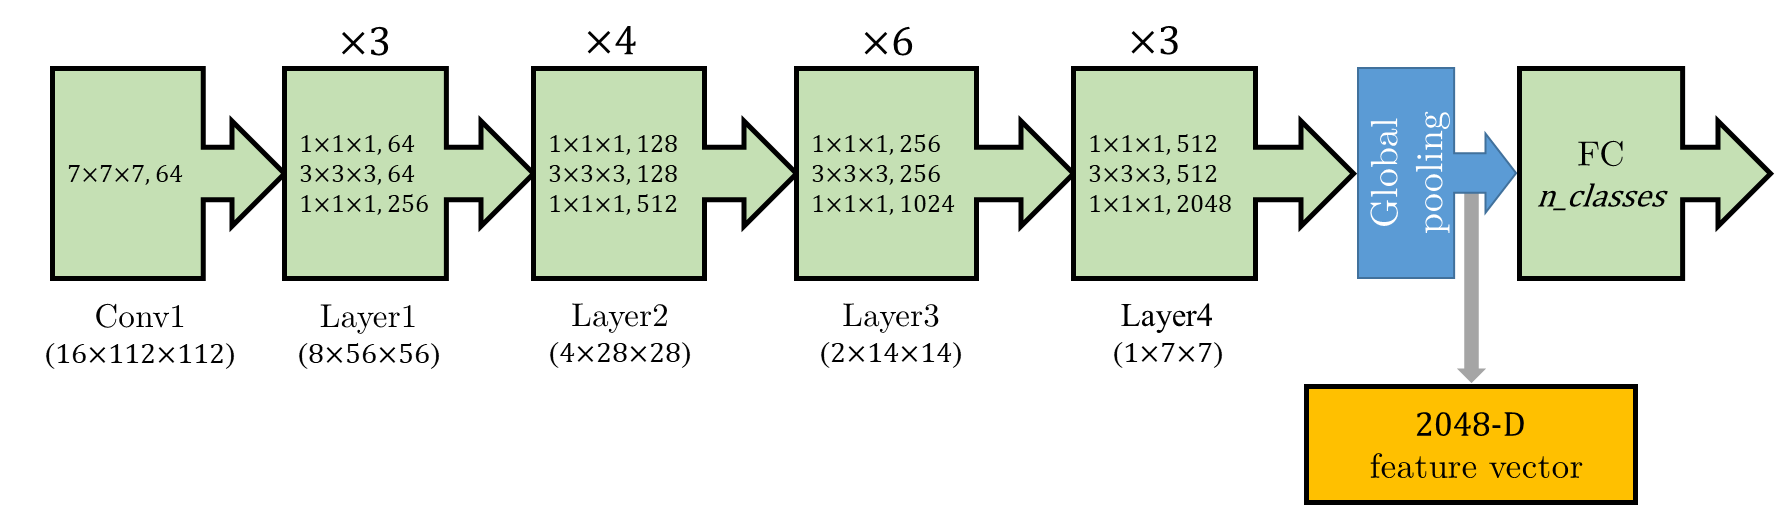
\includegraphics[width=1\linewidth]{Figs/Resnet50_3D.png}
        \caption{Architecture of ResNet-50 3D utilized in this work for feature extraction}
        %\vspace{-0.3cm}
        \label{fig:resnet50_3d}
    \end{figure}

    \textbf{C3D}: 3D deep convolution neural network, which was introduced in \cite{tran2015learning}, has shown to be very efficient for action recognition tasks. C3D takes input as an image sequence instead of a static image, computes the 3D convolution on each 3D cubes from video clip. By doing so, C3D captures both spatial and temporal characteristics of action at the same time.
    \begin{figure}[htbp]
        \centering
        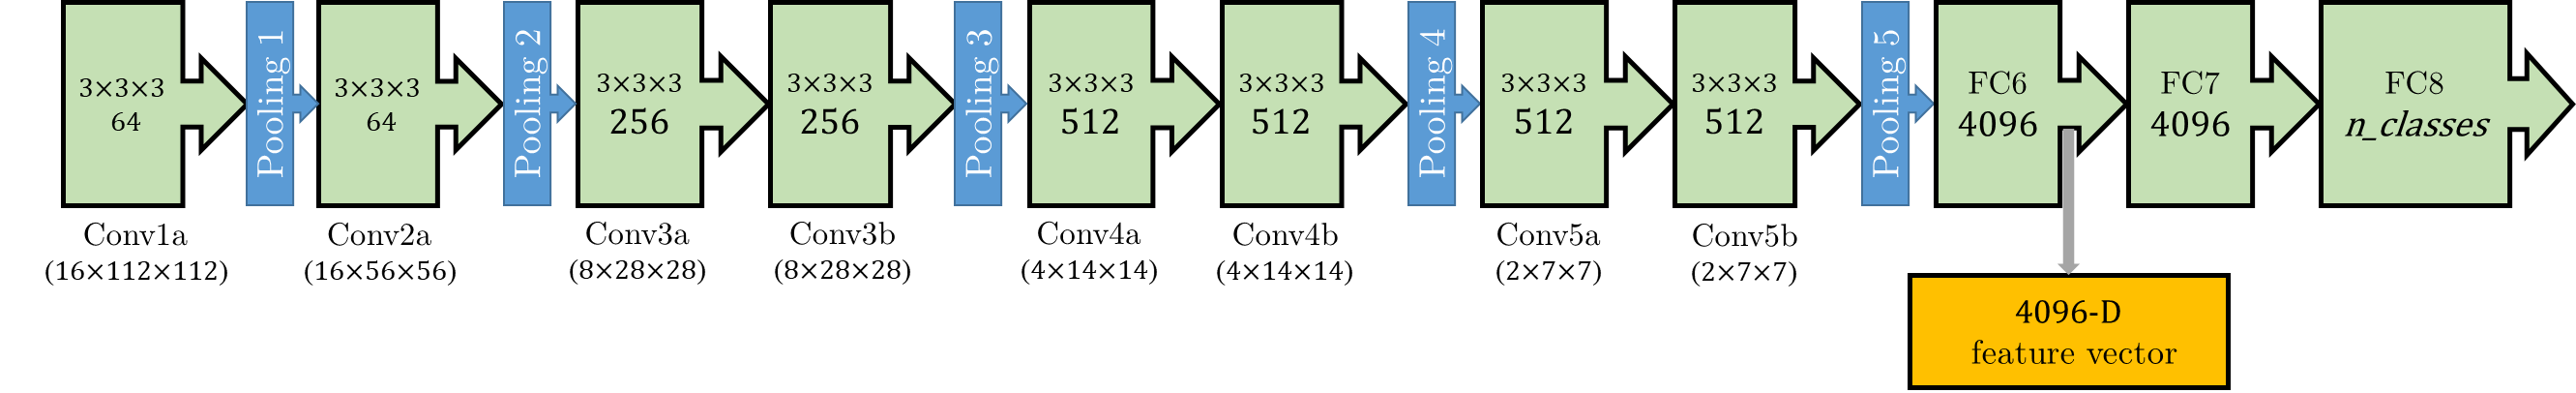
\includegraphics[width=1\linewidth]{Figs/C3D.png}
        \caption{Architecture of C3D utilized in this work for feature extraction}
        %\vspace{-0.3cm}
        \label{fig:C3D}
    \end{figure}
    A C3D network contains 8 convolution, 5 max-pooling and 2 fully connected layers as illustrated in Figure \ref{fig:C3D}. 
    % The number of filters of convolution layers from Conv1 to Conv5 are 64, 128, 256, 512, 512 respectively. All 3D convolution kernels are of size $3\times3\times3$ with stride $1\times1\times1$ and followed by a 3D batch normalization layer. 
    % We utilize the network pre-trained on Sports-1M and fine-tuned on Kinetics dataset.
    The feature vector of 4096 dimensions extracted from FC\-6 layer will be served for training and testing classifiers in further steps.

    To apply in the proposed framework of action and gestures recognition, transfer learning technique is applied for pretrained models on each data stream corresponding to each individual view.
    Details of pre-trained weights and training process of the networks will be presented in Section \ref{sec:experimental_setup}.


    %!TEX root = ../../../main.tex

\section{Construction of common feature space} \label{sec:common}
    %!TEX root = ../../../main.tex

\subsection{Brief summary of Multi-view Discriminant Analysis}
    Suppose that actions belonging to $c$ classes are observed from $v$ views, the number of samples from the $j^{th}$ view of the $i^{th}$ class is $n_{ij}$. We define $X = \{\boldsymbol{x}_{ijk}|i=(1,..,c);j = (1,..,v);k=(1,..,n_{ij})\}$ as samples from $v$ views where 
    $\boldsymbol{x}_{ijk} \in R^{d_j}$ is the $k^{th}$ sample from the $j^{th}$ view of the $i^{th}$ class, $d_j$ is the dimensions of data at the $j^{th}$ view. Here ${\boldsymbol x}_{ijk}$ is a feature vector extracted from the $k^{th}$ sample from the $j^{th}$ view of the $i^{th}$ class. Different methods for features extraction from single view have been presented in previous sections. 

    \textbf{Multi-view discriminant analysis (MvDA)}
    MvDA was an extension of LDA for multi-view scenario \cite{kan2015multi}. It tries to determine a set of $v$ linear transformations to project all action samples from each view $j = (1,..,v)$ to a common space. The projection results of $X$ on the common space is denoted by $Y = \{\boldsymbol{y}_{ijk} = w_j^T\boldsymbol{x}_{ijk}|i=(1,..,c); j=(1,..,v); k=(1,...,n_{ij})\}$. The common space is built by maximizing the between-class variation $\boldsymbol{S}_B^y$ while minimizing the within-class variation $\boldsymbol{S}_W^y$ from all views. $\boldsymbol{S}_B^y$ and $\boldsymbol{S}_W^y$ are computed as follows: 
    \begin{align}
        \boldsymbol{S}_W^y &= \sum_{i=1}^{c}\sum_{j=1}^{v}\sum_{k=1}^{n_{ij}}(y_{ijk}-\boldsymbol{\mu}_i)(y_{ijk}-\boldsymbol{\mu}_i)^T \label{eq:MvDA_Sw}\\
        \boldsymbol{S}_B^y &= \sum_{i=1}^{c}n_i(\boldsymbol{\mu}_i - \boldsymbol{\mu})(\boldsymbol{\mu}_i - \boldsymbol{\mu})^T \label{eq:MvDA_Sb}
    \end{align}
    where $\boldsymbol{\mu}_i=\frac{1}{n_i}\sum_{j=1}^{v}{\sum_{k=1}^{n_{ij}}}{\boldsymbol{y}_{ijk}}$ is the mean of all samples of the $i^{th}$ class from all views in the common space; $\boldsymbol{\mu}=\frac{1}{n}\sum_{i=1}^{c}\sum_{j=1}^{v}{\sum_{k=1}^{n_{ij}}{\boldsymbol{y}_{ijk}}}$ is the mean of all samples of all classes from all views in the common space; $n=\sum_{i=1}^{c}n_i$ is the total data samples from all views.
    Then the objective function is formulated by a Rayleigh quotient:
    \begin{equation}
        (\boldsymbol{\omega}_1^*,\boldsymbol{\omega}_2^*, ..., \boldsymbol{\omega}_v^*) = \operatorname*{argmax}_{\boldsymbol{\omega}_1, \boldsymbol{\omega}_2,..., \boldsymbol{\omega}_v}\frac{trace({S}_B^y)}{trace({S}_W^y)}
        \label{eq:MvDA}
    \end{equation}
    According to \cite{kan2016multi}, the optimization problem could be analytically solved through generalized eigenvalue decomposition. 

    %\textbf{Multi-view discriminant analysis with view consistency (MvDA-vc):}
     In \cite{kan2016multi}, the authors observed that as multiple views correspond to the same objects, there should be some correspondence between multiple views. They then introduce a view consistency constraint into the objective function. The method is called as MvDA-vc. In this paper, we will also compare with MvDA-vc but our method improves the MvDA, so we will not detail MvDA-vc in this section. 
     
     %According to the experimental results presented in the next section, MvDA-vc helps to improves significantly performance of recognition. However, it is difficult to explain explicitly and intuitively how view consitency helpts
     
    %  , that means if $\boldsymbol{X}_j, \boldsymbol{X}_r$ are observed at $j^{th}$ and $r^{th}$ views, then there exists a certain transformation $\boldsymbol{R}$ such that $\boldsymbol{X}_j = \boldsymbol{R}\boldsymbol{X}_r$. As a result, the transformations obtained from two views (i.e. the projection of features extracted from singe view to common view) should have similar relationship: ${\omega}_j = \boldsymbol{R}{\omega}_r$. Let us define $\beta_i$ that captures the structure of the transformation ${\omega}_i$. Then the $\beta_j$ and $\beta_r$ capturing the structures of two transformations of two views $j$ and $r$ should be identical ${\beta}_j = {\beta}_r$.
     
    %  Generalizing to $v$ views, suppose that ${\boldsymbol\beta}_j, j=(1,..,v)$ captures the structures of $v$ transformations ${w}_j$. Following the above observation, the $\boldsymbol{\beta}_r, r=(1,..,v)$ should resemble mutually. That means the similarity between the pair of $\boldsymbol{\beta}_j$ and $\boldsymbol{\beta}_r$ should be minimized. 
    % \begin{equation}
    %      \sum_{j,r=1}^{v}||\boldsymbol{\beta_j} - \boldsymbol{\beta_r}||_2^2
    % \end{equation}
    %  This term is called in \cite{kan2016multi} {\itshape view consistency} and will be added to the denominator of Eq.\eqref{eq:MvDA}
    % \begin{equation}
    % \small
    %     (\boldsymbol{\omega}_1^*,\boldsymbol{\omega}_2^*, ..., \boldsymbol{\omega}_v^*) = \operatorname*{argmax}_{\boldsymbol{\omega}_1, \boldsymbol{\omega}_2,..., \boldsymbol{\omega}_v}\frac{trace({S}_B^y)}{trace({S}_W^y) + \alpha\sum_{j,r=1}^{v}||\boldsymbol{\beta_j} - \boldsymbol{\beta_r}||_2^2} 
    %     \label{eq:MvDA-vc}
    % \end{equation}
    % Similarly, this optimization problem could be analytically solved by relaxing to the ratio trace problem as Eq.\eqref{eq:MvDA}. In the Eq.\eqref{eq:MvDA-vc}, $\alpha$ is an empirically chosen parameter. It puts a weight on the view-consistency assumption. When $\alpha = 0$, the MvDA-vc becomes the original MvDA. 

    %!TEX root = ../../../main.tex

\subsection{Pairwise-covariance Multi-view Discriminant Analysis pc-MvDA}
    MvDA emphasizes on finding a common space with minimal within-class variation while the distances between class means and global mean are jointly maximized. However, the distances between some pairs of classes can be disregarded. In this paper, to obtain this property, we modified MvDA with reformulated between and with-in class scatter matrices terms in a pairwise manner. First, let us define a new inter-class scatter matrix formula that takes paired distance into account:
    \begin{equation}
        \boldsymbol{S}_B^y=\sum_{a=1}^{c}\sum_{b=a+1}^{c}{\left(\mu_a-\mu_b\right)\left(\mu_a-\mu_b\right)^T}
    \end{equation}
    where $a$, $b$ are two distinct classes. For each pairs of class $a$ and class $b$, the between covariance is calculated as:
    \begin{equation}
        {\boldsymbol{S}_B^y}_{ab}={\left(\mu_a-\mu_b\right)\left(\mu_a-\mu_b\right)^T}
        \label{eq:Sb_ab}
    \end{equation}

    The intra-class scatter matrix $\boldsymbol{S}_W^y$ of MvDA is calculated as simple summation of all covariance matrices of each $i^{th}$ class, $i = {1,...,c}$:
    \begin{equation}
        {\boldsymbol{S}_W^y}_i=\sum_{j=1}^{v}\sum_{k=1}^{n_{ij}}{\left(y_{ijk}-\mu_i\right)\left(y_{ijk}-\mu_i\right)^T}
    \end{equation}

    Mathematically, it assumes data samples from each class among all views are identically Gaussian distributed, and contribute evenly to the minimization of intra-class scatter. In reality, it is hardly the case as data variations of samples from different classes and different view points are usually drastically diverse and may also have different dimensions.

    To better represent the distribution of data, pc-MvDA uses a paired intra-scatter matrix which is denoted as
    \begin{equation}
        {\boldsymbol{S}_W^y}_{ab}=\beta\frac{n_a{\boldsymbol{S}_W^y}_a+n_b{\boldsymbol{S}_W^y}_b}{n_a+n_b}+\left(1-\beta\right){\boldsymbol{S}_W^y}
        \label{eq:Sw_ab}
    \end{equation}
    where $0\le\beta\le1$ is a hyper-parameter for regularization between the original global intra-covariance ${\boldsymbol{S}_W^y}$ and the novel two local class covariances ${\boldsymbol{S}_W^y}_a$ and ${\boldsymbol{S}_W^y}_b$. This formulation is closer to the value of covariances of both classes than the standard intra-covariance.

    Instead of solving the vanilla generalized eigen value problem for the whole dataset, we split it into sub-problems for each pairs of class $a$ and $b$, in which we define the objective distance to be minimized between two corresponding classes.
    \textbf{Difference of our proposed method compared to pairwise LDA (pc-LDA)}
    In pc-LDA \cite{kong2014pairwise}, the pairs of $a$ and $b$ classes are regarded as two Gaussian distributions $\mathcal{N}_a(\mu_a,{\boldsymbol{S}_W^y}_a), \mathcal{N}_b(\mu_b,{\boldsymbol{S}_W^y}_b)$ and the objective distance between two classes is defined as their Kullback-Leibler divergence \cite{kullback1951}:
    \begin{equation}
        D_{KL}\left(\mathcal{N}_a\parallel\mathcal{N}_b\right)=\frac{1}{2}\left(\mu_a-\mu_b\right)^{T}{\left({\boldsymbol{S}_W^y}_{ab}\right)}^{-1}\left(\mu_a-\mu_b\right),
    \end{equation}
    Then the final objective is properly weighted to focus on classes with more samples:
    \begin{equation}
        \operatorname*{min}_{\boldsymbol{\omega}_1, \boldsymbol{\omega}_2,...,
        \boldsymbol{\omega}_v}{J}=\sum_{a=1}^{c}\sum_{b=a+1}^{c}{\frac{n_an_b}{{[2D_{KL}\left(\mathcal{N}_a\parallel\mathcal{N}_b\right)]}^q}}
        \label{eq:pc-LDA}
    \end{equation}
    here $q\ge1$ is a hyper-parameter that controls how much the pairs of classes with smaller objective distances are biased over the others.

    In our observation, the minimization of KL divergence for each pairs of classes $a$ and $b$ can be substituted by a generalized eigenvalue problem with the pairwise ${\boldsymbol{S}_W^y}_{ab}$ and the ${\boldsymbol{S}_B^y}_{ab}$ we defined. Although these sub-problems do not have an unified analytical solution to be solved concurrently, the criteria can be formulated in various differentiable ways like in \cite{fukunaga1990441} so we can use gradient descent algorithm:
    \begin{equation}
        J_1=\frac{tr(S_B)}{tr(S_W)};\quad 
        J_2=tr\left(\frac{S_B}{S_W}\right);\quad
        J_3=tr\left|\left|\frac{S_B}{S_W}\right|\right|;\quad
        J_4=\frac{det(S_B)}{det(S_W)}
    \end{equation}

    We choosed the former Fisher loss as the ratio of scalar values is computationally cheaper. Comparing to the objective of pc-LDA in Eq.\eqref{eq:pc-LDA}, our proposed model is obviously more efficient since it contains only simple operators and the need to inverse a singular-prone matrix is negated. Therefore, it is better fit in the scenario where we want to train the model multiple iterations over multi-view high dimensional output.

    Our final objective function of pairwise-covariance multi-view discriminant analysis is sum of all pairwise Fisher criteria with normalized weights:
    \begin{equation}
        \operatorname*{min}_{\boldsymbol{\omega}_1, \boldsymbol{\omega}_2,..., \boldsymbol{\omega}_v}{J}=\sum_{a=1}^{c}\sum_{b=a+1}^{c}{\frac{n_an_b}{n_{cc}^2}{\left[{\frac{trace\left({\boldsymbol{S}_W^y}_{ab}\right)}{trace\left({\boldsymbol{S}_B^y}_{ab}\right)}}\right]}^{q}}
        \label{eq:pc-MvDA}
    \end{equation}
    where $n_{cc}$ is the number of common components as coined in \cite{you2019multi} or simply number of samples in each view. This added normalization term assures that the objective does not depend on size of dataset.

    Let's look at the Fig.\ref{fig:frw}, the nominator of MvDA(-vc) $\boldsymbol{S}_B^y$ is the sum of all distances from mean of every class $\mu_i$, $i = {1,...,c}$ to the mean of all classes $\mu$. This helps to push class far away from the mean of all classes (the dotted green lines in Fig.\ref{fig:frw}). However, it may not ensure that the classes will be far from each other (Fig.\ref{fig:pc-MvDA}a). In this work, we take the pairwise distance into account and integrate them in an multi-view framework (the dotted violet lines in Fig.\ref{fig:frw}). Thanks to this, the classes will be more discriminated (Fig. \ref{fig:pc-MvDA}b). The algorithm for solving pc-MvDA is presented in supplemental materials. 

    \textbf{Illustrative examples:} We illustrate the advantage of pc-MvDA on artificial datasets. Firstly, using function provided by scikit-learn library, we generate several isotropic Gaussian blobs equal to desired number of classes as data samples from one single view. To generate other views, we clone and apply translation, point-wise noise and rotation with random orthogonal group multiplication to the first view.

    In Fig.\ref{fig:synthetic1}, MvDA and pc-MvDA results on 2D synthetic dataset of 180 data points in 2-D space. There are three classes, observed at three viewpoints. We show data distribution and 1-D projection results using MvDA and pc-MvDA respectively. We notice that data points of two classes (the first and the third classes) are close together in original space. When we project in common space by MvDA, these classes are still close together. In contrast, these classes are more discriminant when projected by pc-MvDA.

    Similar to the first example, in the second example, we generate 300 data points of 5 classes observed from 3 different views (Fig.\ref{fig:synthetic2}). We observe that the five clusters of pc-MvDa common space contract strongly and become more separated as compared to the MvDA results (especially the first and the fourth classes).

    \begin{figure}[htbp]
        \centering
        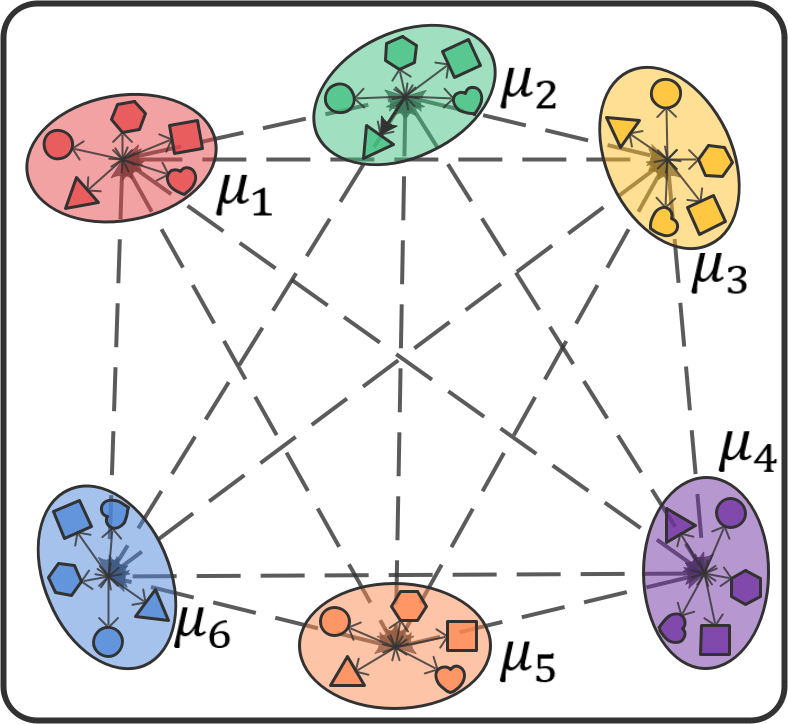
\includegraphics[width=0.7\linewidth]{Figs/pc-MvDA.png}
        \caption{a) MvDA does not optimize the distance between paired classes in common space. b) pc-MvDA takes pairwise distances into account then distinguish better the classes.}
        %\vspace{-0.3cm}
        \label{fig:pc-MvDA}
    \end{figure}

    \begin{figure}[htbp]
        \centering
        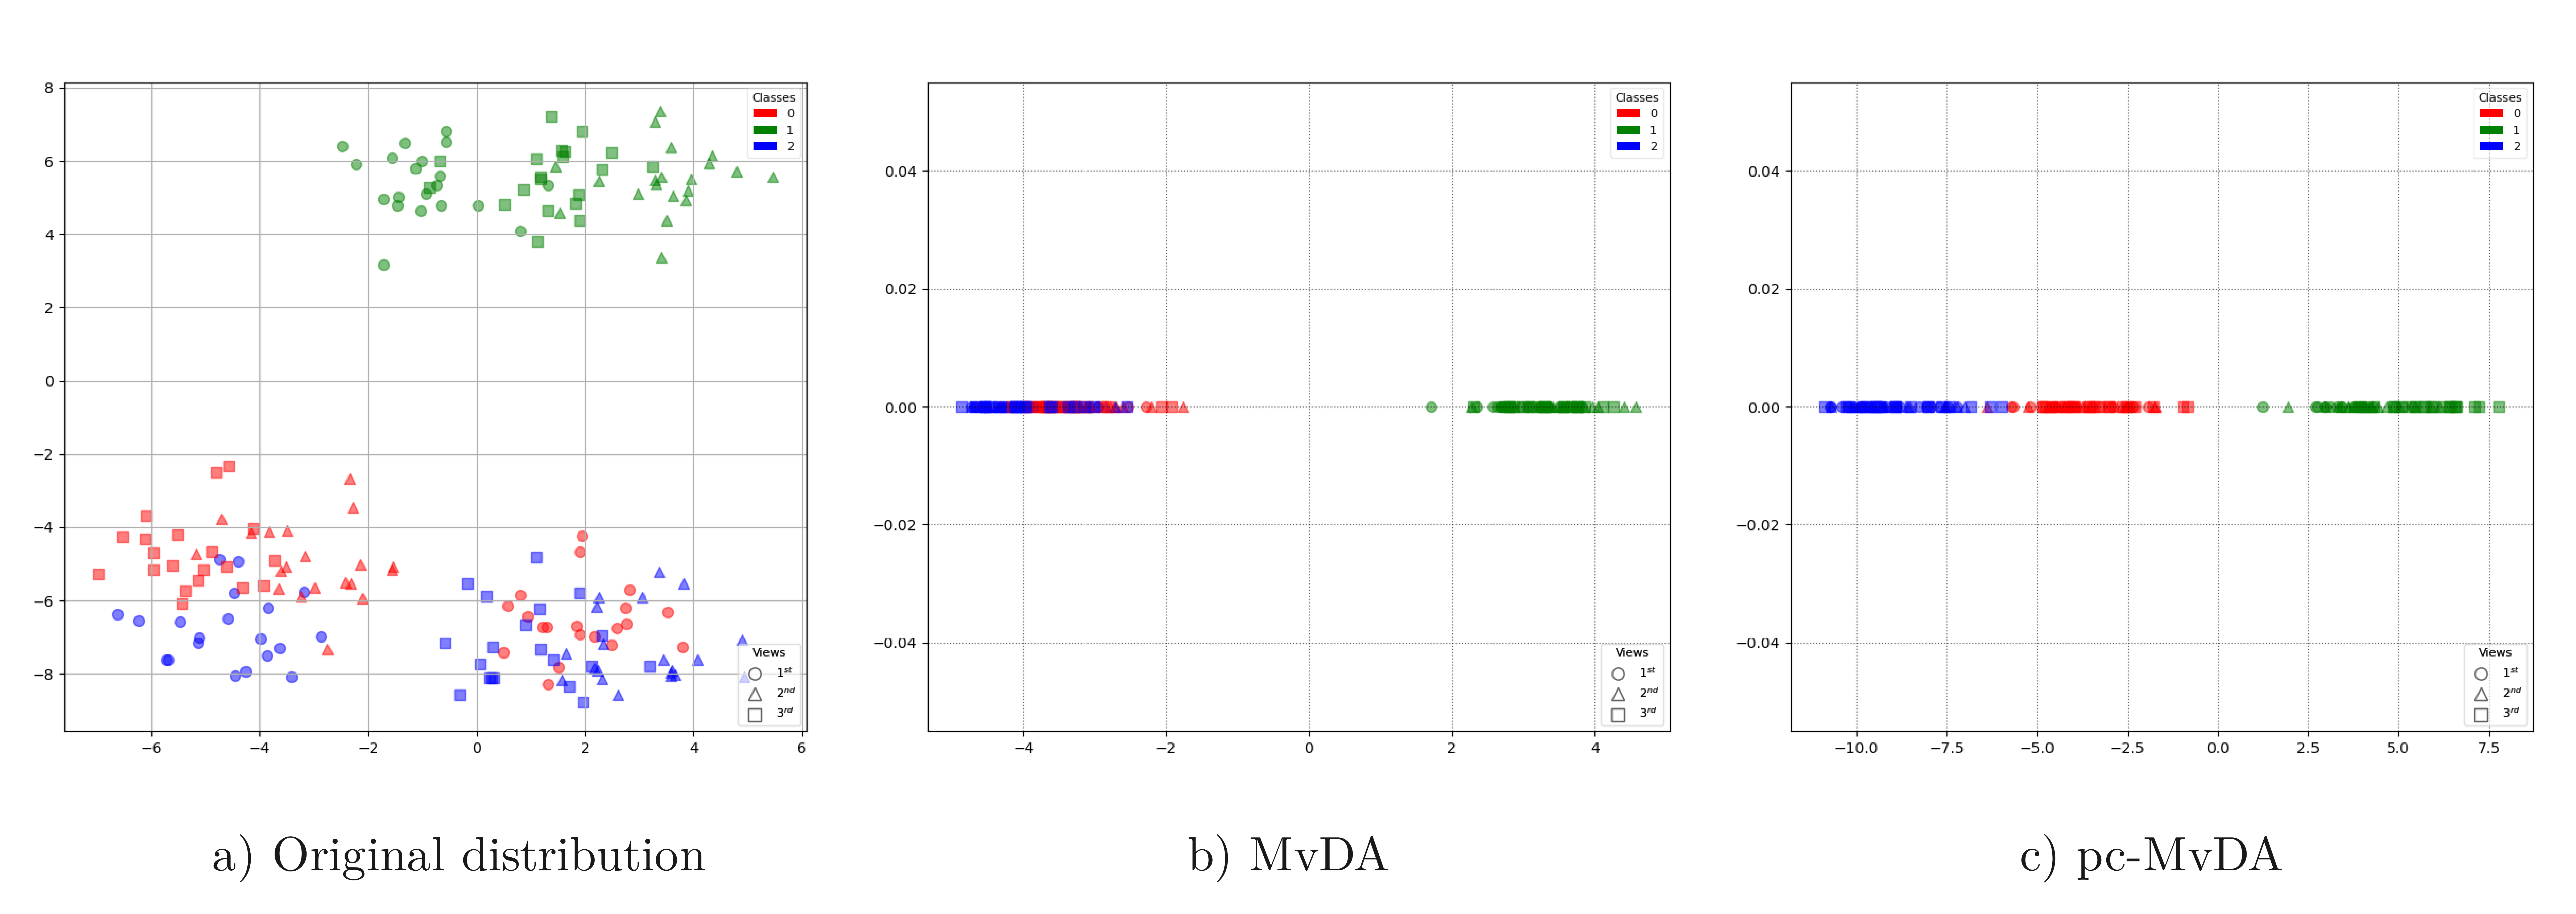
\includegraphics[width=1\linewidth]{Figs/Synthetic1.png}
        \caption{A synthetic dataset of 180 data points, evenly distributed to 3 classes among 3 different views; a) 2-D original distribution; b) 1-D projection of MvDA; c) 1-D projection of pc-MvDA}
        %\vspace{-0.3cm}
        \label{fig:synthetic1}
    \end{figure}

    \begin{figure}[htbp]
        \centering
        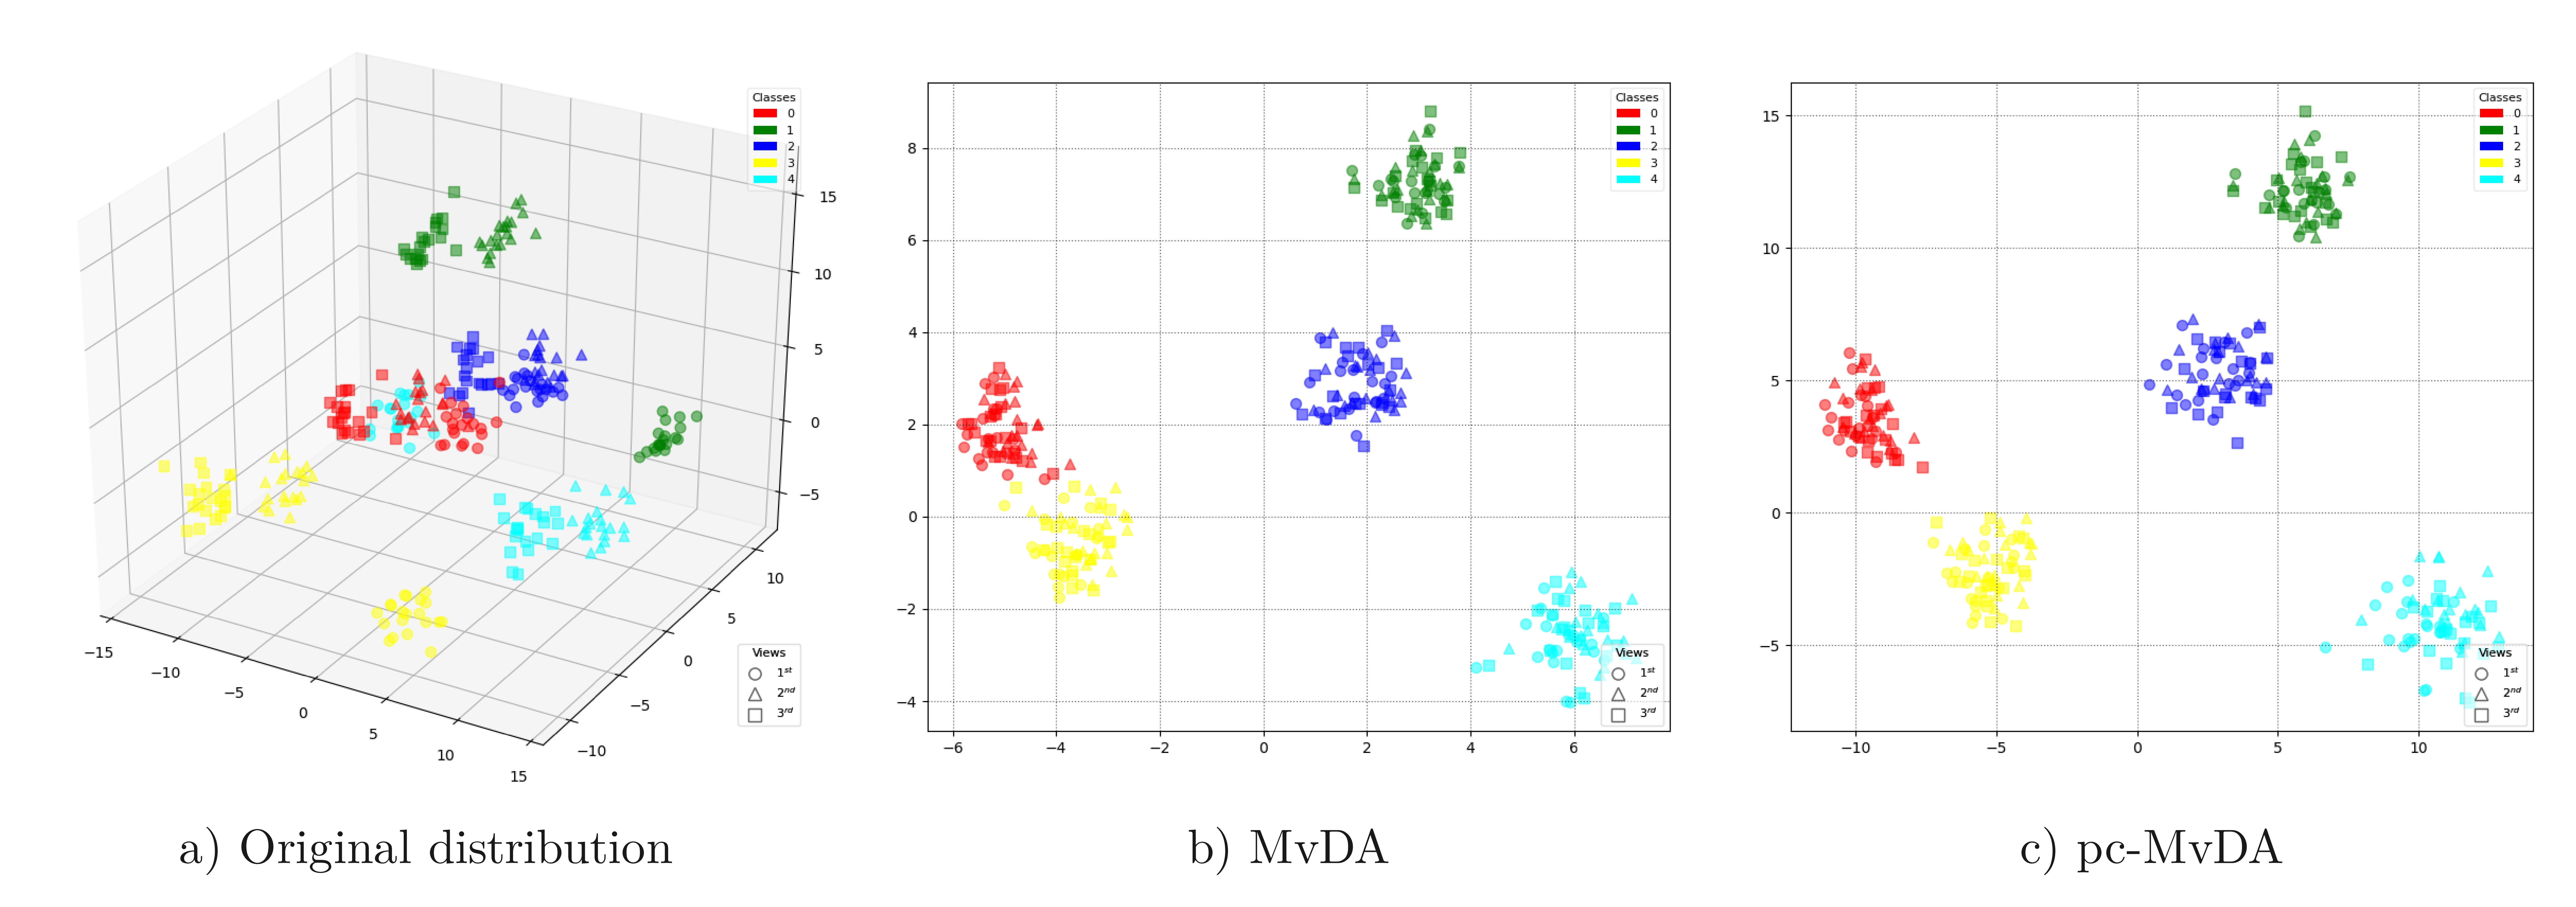
\includegraphics[width=1\linewidth]{Figs/Synthetic2.png}
        \caption{A synthetic dataset of 300 data points, evenly distributed to 5 classes among 3 different views; a) 3-D original distribution; b) 2-D projection of MvDA; c) 2-D projection of pc-MvDA}
        %\vspace{-0.3cm}
        \label{fig:synthetic2}
    \end{figure}



    \section{Summary}
        The novel human action and gesture recognition framework was introduced in this chapter, which consists of two components.
        Firstly, convolutional based clip-level extraction using either 2D CNN (i.e. ResNet) combined with temporal modeling techniques (AP, RNN, TA) or 3D CNN (i.e. C3D, ResNet 3D) are trained separately for each view.
        In the later stage, multi-view analysis algorithms (including pc-MvDA - the main contribution of this thesis) are employed to project common features space, in which the final classification process take place.
        The new formulation of pc-MvDA successfully enforces class separability by adding pairwise distance constraint and casting the final objective to an efficient gradient descent optimization problem that can theoretically be backpropagated to previous layers of CNN feature extractors.
        However, the framework is currently not easily end-to-end trainable due to enormous size of multiple deep feature extractors coupled with the problematic prerequisite of knowing class means when using multi-view analysis as loss function.
